\documentclass[11pt]{beamer}
\usetheme{Dresden}

\usepackage[utf8]{inputenc}
\usepackage[T1]{fontenc}
\usepackage{multicol}
\usepackage{tikz}

\tikzset{
    every overlay node/.style={
        anchor=north west,
    },
}
\def\tikzoverlay{%
    \tikz[baseline,overlay]\node[every overlay node]
}%

\author{Franz Profelt}
\title{Simulation and emulation of realtime communication networks}
\subtitle{Master Thesis}
%\logo{}
%\institute{}
\date{22.06.2016}
%\subject{}
%\setbeamercovered{transparent}
\setbeamertemplate{navigation symbols}{} % disable nav symbols

% left aligned description
\defbeamertemplate{description item}{align left}{\insertdescriptionitem\hfill}

\begin{document}
    \setbeamertemplate{description item}[align left]
    
    \maketitle
    \section{General}

\begin{frame}{General}
    
    \begin{block}{Motivation}
        \begin{itemize}
            \item Urge for testing of embedded systems
            \item Flexible testing scenarios
            \item Improved testing with Emulation and \emph{HiL}
        \end{itemize}
    \end{block}
    
    \begin{block}{Tasks}
        \begin{itemize}
            \item Fundamentals of OMNeT++, simulation, emulation, ...
            \item Design Evaluation
            \item Analysis of the openPOWERLINK stack
            \item Development of an OMNeT++ simulation representing a openPOWERLINK network
        \end{itemize}
    \end{block}
    
\end{frame}
    \section{OMNeT++}
    
\begin{frame}{OMNeT++ Framework}
    \begin{block}{General}
        \begin{itemize}
            \item Object oriented modular discrete event network simulation
            \item Open Source simulation framework written in C++
            \item Discrete event simulation (\emph{DES})
        \end{itemize}
    \end{block}
    
    \begin{block}{Components}
        \begin{itemize}
            \item Network
            \item simple module, compound module
            \item channels
            \item messages, packets
        \end{itemize}
    \end{block}
\end{frame}

\begin{frame}{Simulation core}
    \begin{block}{Scheduler}
        \begin{description}[cRealtimeScheduler]
            \item[cScheduler] standard offline \emph{DES}, baseclass
            \item[cRealtimeScheduler] real-time simulation
            \item[SocketRTScheduler] real-time simulation, emulation with external HTTP client (\emph{sockets} sample)
        \end{description}
    \end{block}
    
    \begin{block}{Parallel simulation}
        \begin{itemize}
            \item Distribution on multiple logical processes (\emph{LP})
            \item Synchronization via specific scheduler
            \item Communication methods (MPI, named pipe, file, ...)
        \end{itemize}
    \end{block}
\end{frame}
    \section{Design}
\begin{frame}{Fundamental Designs}
    \begin{block}{Monolithic}
        \begin{itemize}
            \item Small number of modules
            \item Complex functionality within a single module
            \item Avoiding compound modules
        \end{itemize}
    \end{block}
    \begin{block}{Modular}
        \begin{itemize}
            \item High number of modules
            \item Small functionality within a single module
            \item Combination of multiple modules to compound modules
        \end{itemize}
    \end{block}
\end{frame}

\begin{frame}{Performance Measurement}
    \begin{block}{Measurement Methods}
        \begin{description}[created events]
            \item[runtime] Measurement of the runtime required to simulate a given amount of simulation time
            \item[created events] Measurement Measurement of the number of created events withing a fixed runtime
            \item[real-time] Observation of the real-time simulation indicator (performance ratio) during a parameter sweep for the data generation interval
        \end{description}
    \end{block}
\end{frame}

\begin{frame}{Example Network}
    \begin{block}{Structure}
        \begin{multicols}{3}
            \begin{itemize}
                \item Generator
                \item Dispatcher
                \item Various sinks
            \end{itemize}
        \end{multicols}
    \end{block}
    
    \begin{figure}
        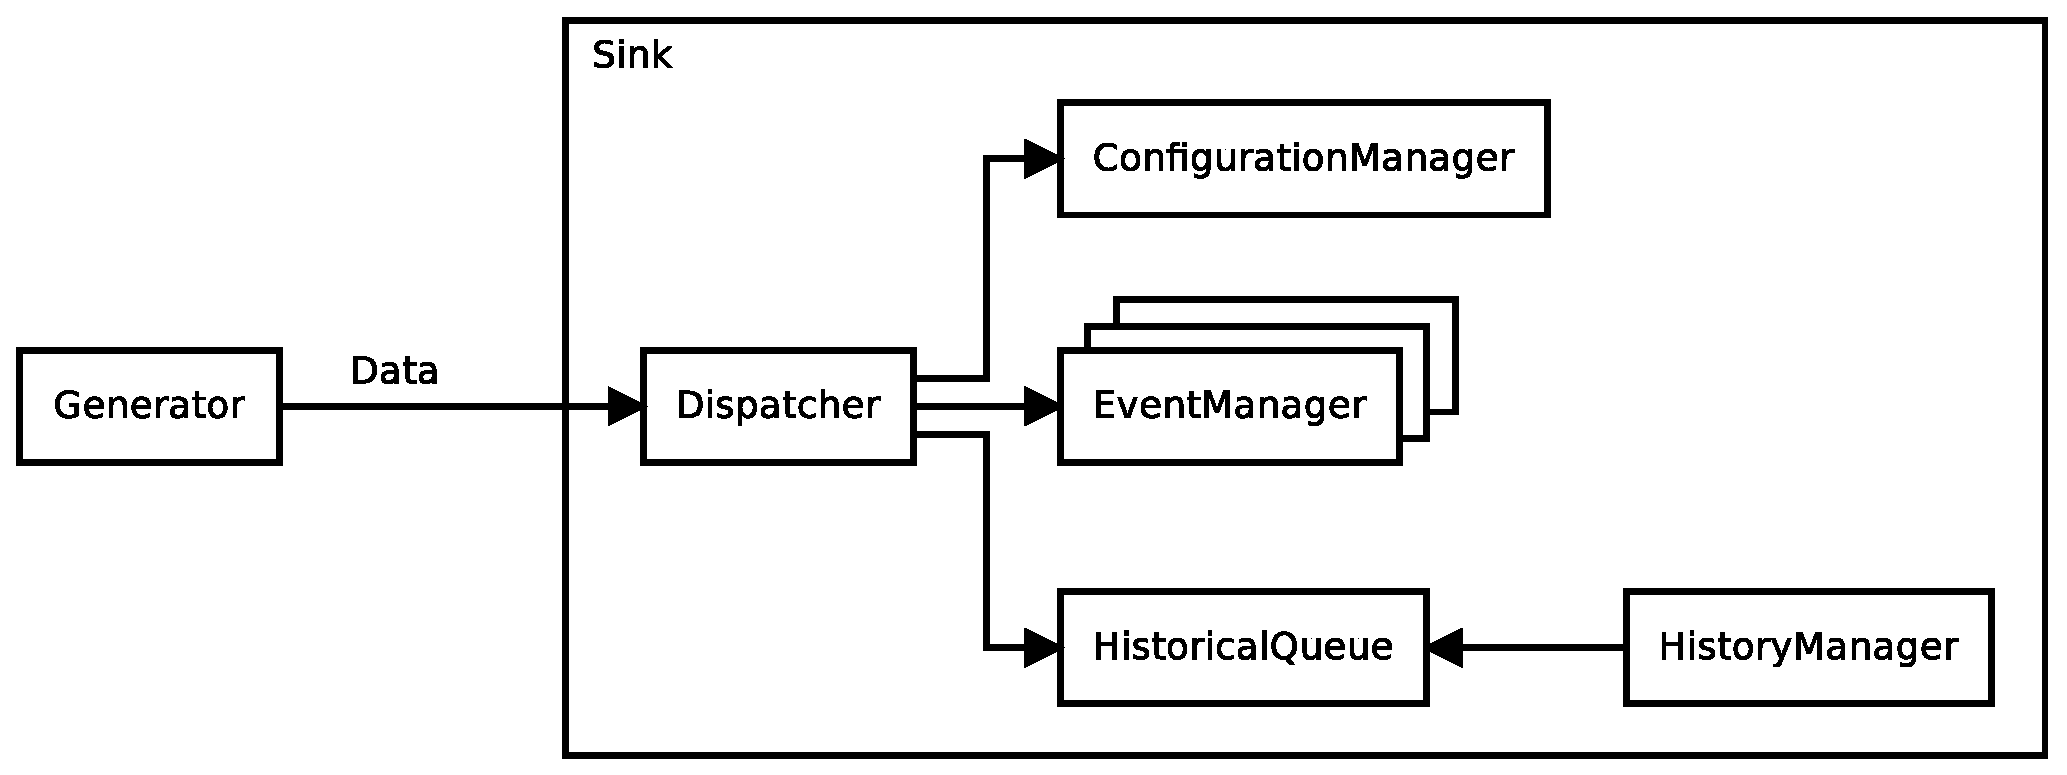
\includegraphics[width=0.9\textwidth]{../../thesis/images/design_test_network.eps}
    \end{figure}
\end{frame}

\begin{frame}{Results}
    The average ratio of performance values using a modular design over a monolithic design.
    \begin{columns}
        \begin{column}{0.48\textwidth}
            \begin{block}{Sequential\strut}
        \begin{description}[created events]
            \item[runtime] $4.033$
            \item[created events] $3.506$
            \item[real-time] $1.592$
        \end{description}
            \end{block}
        \end{column}
        \begin{column}{0.48\textwidth}
            \begin{block}{Parallel\strut}
                \begin{description}[created events]
                    \item[runtime] $2.067$
                \end{description}
            \end{block}
        \end{column}
    \end{columns}
    
    \begin{block}{Conclusion}
        Using a monolithic design as sequential simulation is used for the openPOWERLINK simulation.
    \end{block}
    
\end{frame}
    \chapter{openPOWERLINK}
\label{cha:oplk}
openPOWERLINK is an Open Source implementation of the POWERLINK protocol.
The implementation contains the openPOWERLINK stack, different demo applications for various platforms and is designed for an simple introduction into POWERLINK.
The available project should allow manufacturers an easily integration of POWERLINK into their projects.
The Open Source implementation should targets an improved integration an development of new features.

%TODO general description of openPOWERLINK

\section{POWERLINK}
\label{sec:powerlink}
POWERLINK is an industrial real-time communication protocol based on the IEEE 802.3 standard (Ethernet \cite{ethernet_ieee_2016}).
POWERLINK was developed by the members of the Ethernet POWERLINK Standardization Group (\emph{EPSG}).
The \emph{EPSG} consists of different companies located in the field of real time communications, automation and field bus communication. \cite{epsg_hp}

%TODO general description of POWERLINK

\subsection{Network structure}
\label{sec:oplk_powerlink_network}
A POWERLINK network consists of the following two different node types.

\begin{description}
    \item[MN] The managing node exist once within a normal POWERLINK network and controls the communication flow.
    The MN manages all registered network participants, provides a clock and defines the transmission cycle.
    \item[CN] All other nodes within a normal POWERLINK network are controlled nodes and react according to the controls of the \emph{MN}.
\end{description}

Within a POWERLINK network unique POWERLINK addresses (Node IDs) are assigned to each node.
The address range from 1 to 239 is available for all \emph{CNs} and can be assigned freely.
The address 240 is fixed for the \emph{MN}, each node assigned the Node ID 240 automatically performs the \emph{MN} functionalities.
\cite{epsg_epsg_2013}

A simple POWERLINK network consisting of a \emph{MN} connected to one \emph{CN} directly and additional two \emph{CNs} via a Ethernet HUB is shown in figure \ref{fig:powerlink_network}.

\begin{figure}
    \centering
    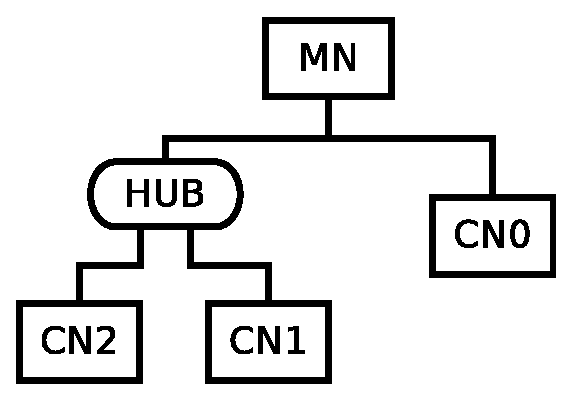
\includegraphics[width=0.5\linewidth]{powerlink_network}
    \caption{POWERLINK network consisting of a \emph{MN} connected to one \emph{CN} and a Ethernet HUB which is connected to two more \emph{CNs}.}
    \label{fig:powerlink_network}
\end{figure}


%TODO describe topologies

\subsection{Frame}
\label{sec:oplk_powerlink_frame}
The POWERLINK frame is embedded in an Ethernet 2 Frames payload and is defined via the Ether type 0x88AB.
Therefore the POWERLINK frame is preceded by the Ethernet 2 Header containing destination \emph{MAC} Address, source \emph{MAC} Address and Ether type.
The payload of an Ethernet 2 Frame can reach up to a length of 1500 bytes succeeding with 4 bytes checksum. \cite[section 3.2]{ethernet_ieee_2016} \cite[section 4.6.1]{epsg_epsg_2013}

In figure \ref{fig:powerlink_frame} the structure of a POWERLINK frame is shown.
The POWERLINK header shown to the left contains the destination and source Node Id preceded by the message type.
The payloads length and content is depending on the transmitted message and thereby defined by the message type. \cite[section 4.6.1.1]{epsg_epsg_2013}

\begin{figure}
    \centering
    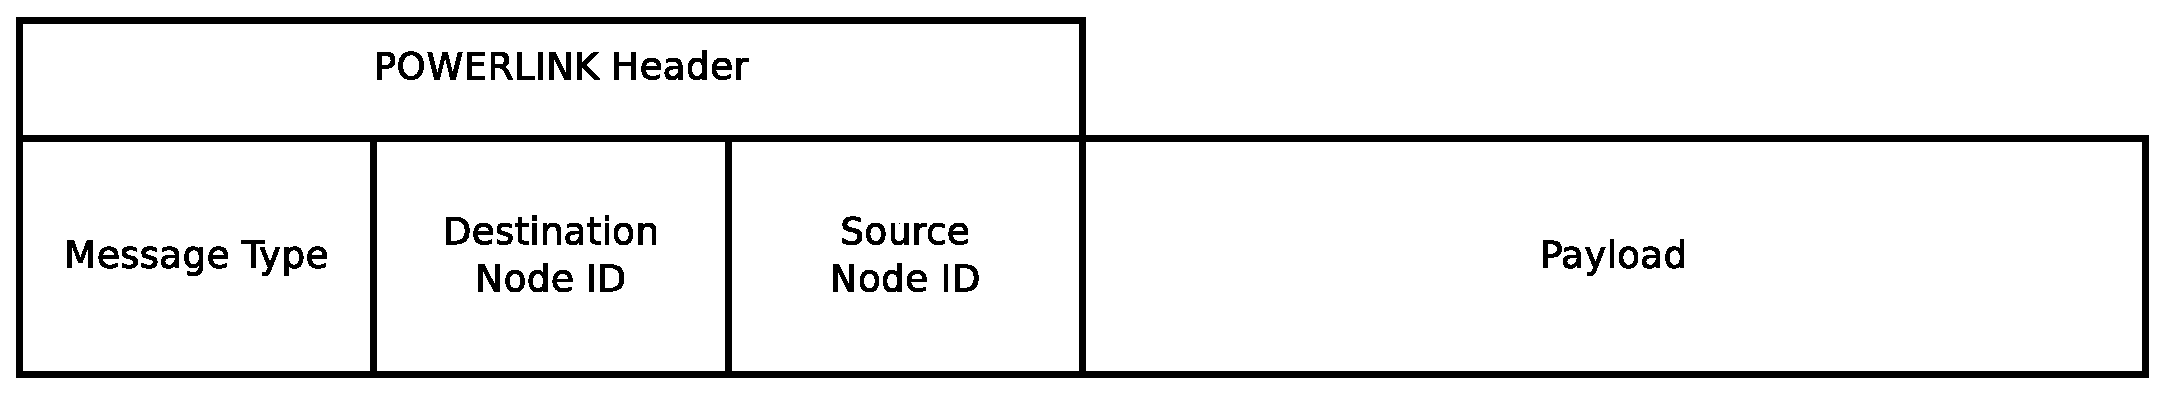
\includegraphics[width=0.9\linewidth]{powerlink_frame}
    \caption{POWERLINK frame showing POWERLINK header and payload.}
    \label{fig:powerlink_frame}
\end{figure}

Detailed information about the different structures of transmitted payloads depending on the message type can be found here \cite[section 4.6.1.1.1]{epsg_epsg_2013}

\subsection{Commands}
\label{sec:oplk_powerlink_commands}

As mentioned above different transmitted POWERLINK messages are defined via the message type.
The following commands are distinguished by the according message type.

\begin{description}
    \item[Soc] Start of cycle is sent by the \emph{MN} as multicast and defines the start of the POWERLINK cycle and the isochronous phase.
    \item[PReq] Poll request is sent by the \emph{MN} to a specific \emph{CN} transmitting data and requesting the transmission data from the \emph{CN}.
    \item[PRes] Poll response is sent by the \emph{CN} as multicast as response to a \emph{PReq} and contains data from the \emph{CN}.
    \item[SoA] Start of Asynchronous is sent by the \emph{MN} as multicast and defines the end of the isochronous phase and the begin of the asynchronous phase.
    \item[ASnd] Asynchronous send is sent either by the \emph{MN} or a \emph{CN} as multicast and contains asynchronous data.
\end{description}

The sequence of sent command within a POWERLINK cycle is shown in the next section.

\subsection{Communication cycle}
\label{sec:oplk_powerlink_commcycle}

The POWERLINK communication cycle is separated in two different phases.

The isochronous phase is the first part of a POWERLINK cycle and is started by the \emph{MN} sending a \emph{SoC} message.
Within this phase the \emph{MN} is polling each \emph{CN} with registered isochronous data.
This polling is accomplished via sending \emph{PReq} message to each \emph{CN}.
This message includes information for the \emph{CN} and also isochronous data which should be sent from the \emph{MN} to the specific \emph{CN}.
After the reception of the \emph{PReq} message the \emph{CN} is sending a \emph{PRes} message as multicast.
This message includes all isochronous data which is requested by the \emph{MN} or any other \emph{CN}.
By multicasting this message each node which should receive a specific data set is immediately receiving the new values. \cite[section 4.2.4.1.1]{epsg_epsg_2013}

When the last isochronous \emph{CN} sent its \emph{PRes} message the isochronous phase is over.
The end of this phase and the start of the asynchronous phase is marked by the sent \emph{SoA} message by the \emph{MN}.
This message contains information about the node which is assigned to the current asynchronous slot.
In each cycle the \emph{MN} assigns the asynchronous slot to either itself or to a \emph{CN}.
Additionally the requested service is transmitted.
Demands a \emph{CN} the assignment to a asynchronous slot this must be communicated to the \emph{MN} either by the \emph{PRes}, \emph{IdentResponse} or \emph{StatusResponse} message.
The communicated number of pending asynchronous messages can additionally provide a priority for better scheduling. \cite[section 4.2.4.1.2]{epsg_epsg_2013}


In figure \ref{fig:powerlink_cycle} a simple POWERLINK communication cycle is shown.
Above the horizontal time axis all command sent by the \emph{MN} are shown.
Commands sent by different \emph{CNs} are displayed below the axis.
This communication cycle shows the isochronous phase marked by the dotted box to the left.
This phase includes the starting command \emph{SoC} and the sequential polling of each \emph{CN}.
This example matches the shown network in figure \ref{fig:powerlink_network} and contains three \emph{CNs}.
The different \emph{CNs} are immediately responding to the polling request.

At the right side in figure \ref{fig:powerlink_cycle} the asynchronous phase is marked by the dashed box.
The asynchronous phase contains the \emph{SoA} command  and following asynchronous data transmission.

\begin{figure}
    \centering
    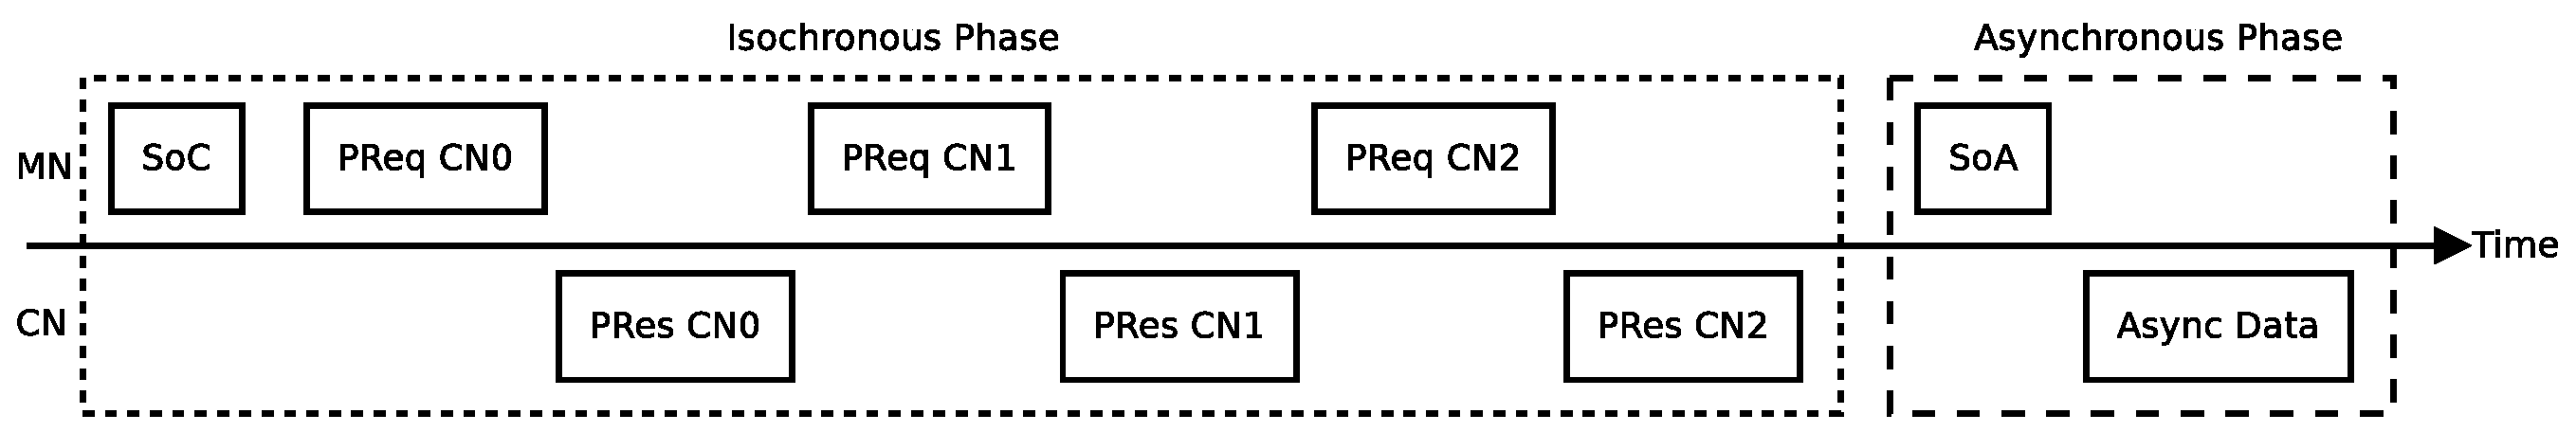
\includegraphics[width=0.95\linewidth]{powerlink_cycle}
    \caption{POWERLINK communication cylce containing Isochronous Phase with polling of three \emph{CNs} and Asynchronous Phase.}
    \label{fig:powerlink_cycle}
\end{figure}

\subsection{Data transmission}
\label{sec:oplk_powerlink_data}


\section{Structure}
\label{sec:oplk_structure}
The openPOWERLINK stack distribution package is structured in different main directories containing demo applications, documentation, driver implementation, the stack sources and multiple more.

For this paper the most important parts are the stack sources and demo applications..
Furthermore an additional simulation directory will be added whose content will be discussed in section \ref{sec:porting_simstub_sim}.

The \emph{apps} folder contains different demo application for embedded targets, linux and windows operating systems.
These demo applications contain exemplary implementations of \emph{MNs} and \emph{CNs}.
These application are analyzed and ported to demo applications within OMNeT++ in the section \ref{sec:porting_demo}.

\subsection{stack folder}
\label{sec:oplk_structure_stack}
The stack folder contains the following structure. \cite{openpowerlink_doc} %TODO: refine citation
\begin{description}
    \item[build] build directory for output files of the build process.
    \item[cmake] configuration files for the build toolchain.
    \item[include/oplk] represents the main include directories for all applications using the openPOWERLINK stack.
    \item[include/common] represents a common internal include directory.
    \item[include/kernel] represents an internal include directory for kernel modules.
    \item[include/target] represents an internal include directory with target specific files.
    \item[include/user] represents an internal include directory for user modules.
    \item[lib] represents the installation directory for the openPOWERLINK libraries.
    \item[proj] represents the directory containing different library projects.
    \item[src/arch] represents a source directory with architecture specific functions.
    \item[src/common] represents a source directory with sources for user and kernel layer.
    \item[src/user] represents a source directory with sources for the user layer.
    \item[src/kernel] represents a source directory with sources for the kernel layer.
\end{description}

This structure represents the architecture of the openPOWERLINK stack, which is explained in the following section.

\subsection{Architecture}
\label{sec:oplk_structure_architecture}

The openPOWERLINK stack is generally separated in kernel and user layer.
This separation was introduced with the version 2.X of the openPOWERLINK stack and is detaching the higher level user functionalities from the lower level kernel functions including time critical behavior and hardware access.

The user and kernel layer are separated by the communication abstraction layer (\emph{CAL}).

%TODO explain architecture including user, kernel, CAL, AMI, HAL, ...
%TODO figure with system overview

\subsection{Configuration and build}
\label{sec:oplk_structure_build}

%TODO rework
The build tool \emph{CMAKE} is used for dynamic creation of according makefiles using definitions and special sources for platform dependency.

Within the openPOWERLINK folder structure the main \emph{CMAKE} file \emph{CMakeLists.txt} checks the current \emph{CMAKE\_SYSTEM\_NAME} variable and creates the according makefile.
The subfolder cmake the general and platform specific cmake-files are located.
The general files \emph{directories.cmake} and \emph{stackfiles.cmake} are always included in the generation process.

Within \emph{directories.cmake} the location of the source, include, user-, kernel-space, architecture files are defined.
The \emph{stackfiles.cmake} file contains the definitions for specific source files grouped in categories like \emph{event}, \emph{cal} and many more.
The platform specific source files are also defined within this file with the according names.

The global \emph{CMAKE} file loads according to the \emph{CMAKE\_SYSTEM\_NAME} and \emph{CMAKE\_SYSTEM\_PROCESSOR} variable the correct system specific options file.
This option file includes options for enabling and disabling part of the openPOWERLINK stack.
For example the generation of the \emph{CN} or \emph{MN} library can be en- or disabled.
Further options are platform specific and provide configuration possibilities for specific usages.

Checking the defined options the according projects are included in the generation and later on the build process.
These projects are located in the \emph{proj} folder.


\subsection{\emph{Proj} folder} %TODO check is useful
\label{sec:oplk_structure_proj}
The \emph{proj} folder contains different directories for three target systems:

\begin{description}
    \item[generic] contains projects for embedded targets without underlying operating systems.
    Providing implementations of \emph{MN} and \emph{CN} for different targets.
    \item[linux] contains projects for linux operating systems using different technologies (Kernel Module, dirver, ...).
    \item[windows] contains projects for windows operating systems using different technologies (Kernel Module, dirver, ...).
\end{description}

Within a specific target folder the different projects are located.
For example the projects \emph{liboplkmn} and \emph{liboplkcn} exist for windows and linux systems.
The different projects represent either different functionalities or different targets and included technologies.

Specific files for each project are located in each folder, including a \emph{CMakeListst.txt} file.
This is included by the according option files.
Within these \emph{CMakeListst.txt} file the specific source files are gathered and set within variables like \emph{LIB\_SOURCES}.
These variables are used for defining the build targets.
The type, location and additional libraries are also either defined within the project files or the option files.

The build targets mostly are libraries which can be linked to the resulting application.

\section{Platform dependency}
\label{sec:oplk_platform}
%TODO: rework and enhance
As described in section \ref{sec:oplk_structure} the configuration and build process defines the according platform specific implementations and libraries.

For platform specific functionalities the implementation of the openPOWERLINK stack uses common header files with specific implementations.

For defining which implementations are platform specific the \emph{CMAKE} file \emph{stackfile.cmake} is analyzed.

The following modules are implemented platform dependent:

\begin{description}
    \item[oplkinc.h] provides macros for target specific functions which depends on the targeting platform or operating systems.
    Defined are small standard functions regarding memory operations.
    \item[Trace] module providing a function for tracing the execution.
    \item[\emph{OBD} configuration] containing specific for functions for storing and restoring of the \emph{OD}.
    The implementation is split in functions regarding file operations and a generic cyclic redundancy check (\emph{CRC}) calculation.
    \item[\emph{SDO} via \emph{UDP}] this implementation contains the transmission of \emph{SDO}s via user datagram protocol (\emph{UDP}).
    The specific implementations provide usage of operating system calls of linux and windows or the usage of a generic header \emph{socketwrapper.h} which allows the implementation for other targets.
    \item[\emph{CAL}] includes different interfaces for the user and kernel space for each containing module (control, \emph{DLL}, \emph{PDO}, error handler, event).
    \item[Timer] providing functions for setting timer.
    \item[Circular buffer] providing the system specific functionalities used within the \emph{circular\_buffer} as creation, allocation, deallocation, locking, connecting and disconnecting.
    \item[Memmap] providing an interface for the memory mapping library used for memory mapped communication in between kernel and user space.
    \item[Target] providing an interface for target specific functions as sleep, interrupt control, tick and implementations of locks and mutexes.
    \item[\emph{AMI}] providing an interface for architecture specific memory functions.
    \item[Edrv] represents the Ethernet driver which is communicating with the used Ethernet media access control (\emph{MAC}) controller.
\end{description}

The porting ot the described platform dependencies to the OMNeT++ simulation environment and the according analyzes are described in the following chapter.
    \chapter{Simulation}
\label{cha:simulation}

A Simulation attempts to replicate and forecast the behavior of real world systems.
Such a replication is used in various fields for testing and verifying theories and systems.
The field of simulation steadily gains importance, due to the increasing complexity of systems; e.g. embedded systems and real-time systems.
Especially the development and testing of real-time communication systems can essentially be improved by using simulation and emulation techniques.

Different types of simulation are applicable for different types of simulated systems and aimed results.
Differences are shown in the processing of the simulated systems and in the handling of simulation time.
\cite[section 1.2]{mchaney2009understanding}

\section{Continuous simulation}
\label{sec:simulation_cont}
Continuous simulations handle uninterrupted values over a simulated time range.
This behavior may be determined by equations describing the system.
For correct simulation of a continuous system the model must be executed for the whole simulated time range.
These simulations are usable for scenarios when the temporal behavior of the simulated models is of interest. \cite[section 1.2.1]{mchaney2009understanding}

Simulations and testing scenarios in the field of real-time communication are based on discrete events at specific points in time, e.g. the reception of data.
The continuous processing of occasions between events is often not necessary, therefore a discrete event simulation (\emph{DES}) is more applicable.

\section{Discrete event simulation}
\label{sec:simulation_event}
This type of simulation is based on processing discrete events.
During the processing of events the simulation time does not advance and the required processing time is not considered in simulation time.
The simulation time is advancing with multiple processed events and their defined point in simulation time.
Between two consecutive events neither any processing is done nor changes of the system state are occurring. \cite[chapter 1]{matloff_introduction_2008}

The assumption is that none, for the simulation relevant, events are happening between two consecutive events.
This exclusion is done by the implementation of the simulated model and must be concluded with care to the intention of simulation.
Simulating a real world system therefore requires the filtering of occasions for focusing on the simulation goal. \cite[section 4.1.1]{omnet_manual}

The implementation of a \emph{DES} can be done in various ways using different strategies or paradigms.
In \cite[chapter 2]{matloff_introduction_2008} Matloff introduced different paradigms to realize a \emph{DES}.
Using OMNeT++ the \emph{Event-Oriented Paradigm} and the \emph{Process-Oriented Paradigm} are applicable and can be achieved as following:

\begin{itemize}
    \item The usage of the \emph{handleMessage} method matches the \emph{Event-Oriented Paradigm} and allows event based development.
    \item The \emph{Process-Oriented Paradigm} can be realized by using the \emph{activity} method and represents the \emph{process style} strategy.
\end{itemize}

\begin{sloppypar}
The \emph{Activity-Oriented Paradigm} could also be implemented within OMNeT++ by using either the \emph{activity} or the \emph{handleMessage} method.
This paradigm would require the implementation of a custom polling module which checks regularly for new events or monitors the activity of other modules.
This implementation would replace and bypass the handling and scheduling of messages in OMNeT++ and is not recommended. \cite[chapter 2.1]{matloff_introduction_2008}
\\
\end{sloppypar}

The above discussed types of simulations belong to the group of \emph{offline simulations} i.e. the simulation time is not connected to the processing time.
Approaching the fields of emulation and \emph{HiL} such a connection is necessary and the behavior of \emph{offline simulations} is unusable.
These fields demand the type of real-time simulation.  \cite[section III.B]{belanger_what_2010}

\section{Real-time simulation}
\label{sec:simulation_real_time}
Real-time simulations change the meaning of simulation time and add a connection to the real-time.
The simulated events should be executed at the correct time to match the real-time.
In this context the real-time represents the real world time, cpu time, or wall time, i.e. the time which passes for the real world during the execution of the simulation.
Running a real-time simulation results in processing a simulated second within an elapsed real world second.
This type of simulation is not possible for every simulated system as the limits are defined by the time required to execute the operations specified by the model.

The achieved execution speeds are strongly depending on the following factors:
\begin{description}
    \item[Model] The complexity of the simulated model, i.e. the functionality to process events affects the achievable execution speed.
                 Simple functionalities can be executed faster than complex library calls or nested functions.
    \item[Host system] The properties of the host system used for running the simulation define the possible execution capabilities and therefore the performance of the executed simulations.
                       This dependency is described in section \ref{sec:simulation_requirements}.
\end{description}

If the execution of the model behavior for reacting to an event takes more processing time than the simulated duration (timespan to next event), the simulation lags behind the real world behavior.
Such an erroneous behavior must be corrected by the simulation core by speeding up the simulation, for example by decreasing idle times between events.
The correction of such behavior results in an increased jitter (variance of event execution time).
\cite[section III.B]{belanger_what_2010}

The quality of the real-time simulation is strongly depending on the simulated system and its composition.
Therefore the ideal results can be achieved by analyzing the simulated system regarding the real-time requirements and processed events.
An example of such an analysis and the modifications of an OMNeT++ simulation for timing improvements are shown in \cite{scussel_improvements_2015}.

The existing functionalities and properties of a simulation using the OMNeT++ framework is shown in the next section.

\section{Simulation with OMNeT++}
\label{sec:simulation_omnet}
By default simulations developed with OMNeT++ are discrete event based simulations.
This behavior is defined by the scheduler and the simulation core, which can be tailored by using custom components. \cite[section 4.1]{omnet_manual}

Within OMNeT++ each event is represented by a message with a defined \emph{arrival time}.
Events are created by modules and then inserted in the so called future event structure (\emph{FES}).
The simulation core executes all events within the \emph{FES} at the according simulation time.

The scheduler is the main part of the simulation core for controlling the event handling the execution order.
The scheduler accesses the \emph{FES} and chooses the next event to be handled by the simulation.
The class \emph{cScheduler} represents the interface which is required for an event scheduler usable in OMNeT++.
By default the derived class \emph{cSequentialScheduler} is used.
This scheduler implements the default discrete event based simulation and handles the events according to their execution time, scheduling priority and scheduled time.
The scheduling priority provides a mechanism for controlling the execution order of multiple events at the same time. \cite[section 4.1]{omnet_manual}.

An exemplary approach to realize the type of real-time simulation is implemented in the \emph{cRealTimeScheduler}.
This scheduler executes the events according to their planned arrival time.
The arrival time of the next event is compared with the current real time.
When the simulation is ahead of the real time, the simulation is paused for the remaining time.
The \emph{cRealTimeScheduler} waits in hard-coded 100 ms chunks for allowing a responsive simulation including graphical updates.
This provided scheduler does not handle a lagging simulation in a special way and simply skips the waiting times within the method \emph{getNextEvent}. 
The definition and implementation of the \emph{cRealTimeScheduler} are shown in the appendix section \ref{app:omnetpp_code_real_time_scheduler} or in the OMNeT++ API \cite[cRealTimeScheduler]{omnet_api}.

For emulations and \emph{HiL} this concept is not applicable, because the communication with real components does rarely contain static sleep times.
The OMNeT++ sample \emph{sockets} demonstrates this problem and a possible solution with a custom scheduler implementing the \emph{cScheduler} class.
The custom scheduler \emph{SocketRTScheduler} and its functionality is further analyzed in section \ref{sec:emulation_omnet_existing}.

% omnet++ real time handling/correction
Handling a simulation which is faster than the real world system can be done in various ways as demonstrated by \emph{cRealTimeScheduler} or the \emph{SocketRTScheduler}.
If the simulation is lagging behind the real-time, the scheduler must try to speed up the simulation and catch up to the real time.
The task of catching up to the real-time is very difficult for complex simulations with tight timings.
If the simulation lags constantly behind the real world using the \emph{cRealTimeScheduler} it becomes a discrete event based simulation and no real-time simulation is possible.

The sample scheduler provided by \emph{cRealTimeScheduler} and \emph{SocketRTScheduler} can lead to the correct strategy of implementing an optimized scheduler.

To validate a real-time simulation regarding timing quality the performance ration can be used.
This ratio represents the simulated seconds per real time seconds.
A lagging simulation is defined by a performance ratio of less than one and simulation which simulates faster as the real time shows a ratio greater one.
The goal of a real time simulation is a constant ratio of one.
The process of catching up of a lagging simulation to achieve a performance ratio of one can also influence the general timing behavior.
Therefore the variation of delays (jitter) increases when the simulation lags temporarily.
For emulations or the fields of \emph{HiL} an increased jitter for a signal can be very critical and must be analyzed carefully.

The host machine for the simulation and its components affect the achieved simulation times.
The dependencies of the host system and the results of existing researches is shown in section \ref{sec:simulation_requirements}.

Developing the simulation of a given system results in the situation of existing code.
This code must be encapsulated in different modules and be executed depending for incoming messages and thereby creating new message for sending.
Given systems can be designed in various hierarchies in sight of number of modules and complexity of simple modules.
The different designs and their effects on real time simulation is shown in the chapter \ref{cha:design}.

\section{System requirements}
\label{sec:simulation_requirements}
The host system for the simulation is very important regarding speed and performance of a simulation and therefore the achievable timings of a real-time simulation.
The limitations of achievable timings of a real-time simulations are defined by the execution speed of the simulated model plus the time for executing the simulation functionality around it.
Assuming the \emph{RAM} (random access memory) of the host systems is large enough to hold the complete simulation code and data, the limit is defined by the execution speed of the code.
Which is affected by the \emph{CPU} (central processing unit) capabilities and the speed of connected memories.
These memories include the \emph{RAM}, every cache and register which is used for holding simulation code and data.
The evolution of simulations and real-time simulations arises from analog simulations, to digital simulations running on supercomputers and currently common simulations running on commercial of the shelf (\emph{CTOS}) systems and field programmable gate arrays (\emph{FPGA}).
This evolution provides more computing capabilities for lower costs. \cite[section IV]{belanger_what_2010}
    
    % end frame
    \bgroup
    \setbeamercolor{background canvas}{bg=black}
    \begin{frame}[plain]{}
    \end{frame}
    \egroup
\end{document}